% ══════════════════════════════════════════════════════════════════
% LICITRA Technical Report Series
% Report No. LICITRA-TR-2026-02
% LICITRA-SENTRY — Version 0.1, March 2026
% ══════════════════════════════════════════════════════════════════
\documentclass[11pt,a4paper]{article}

% ── Packages ──────────────────────────────────────────────────────
\usepackage[margin=1in]{geometry}
\usepackage{amsmath,amssymb,amsthm}
\usepackage{booktabs}
\usepackage{hyperref}
\usepackage{xcolor}
\usepackage{graphicx}
\usepackage{enumitem}
\usepackage{fancyhdr}
\usepackage{tikz}
\usetikzlibrary{arrows.meta,positioning,shapes.geometric,fit,calc}
\usepackage{tabularx}
\usepackage[T1]{fontenc}

% ── Hyperref Setup ────────────────────────────────────────────────
\hypersetup{
  colorlinks=true,
  linkcolor=blue!60!black,
  citecolor=blue!60!black,
  urlcolor=blue!60!black,
  pdftitle={LICITRA-SENTRY: Deterministic Inter-Agent Authorization
            Control Plane with Cryptographic Audit Integrity},
  pdfauthor={Narendra Kumar Nutalapati},
}

% ── Header / Footer ──────────────────────────────────────────────
\pagestyle{fancy}
\fancyhf{}
\fancyhead[L]{\small LICITRA-TR-2026-02 \quad v0.1}
\fancyhead[R]{\small Nutalapati (2026)}
\fancyfoot[C]{\thepage}
\renewcommand{\headrulewidth}{0.4pt}

% ── Theorem Environments ──────────────────────────────────────────
\newtheorem{theorem}{Theorem}[section]
\newtheorem{property}[theorem]{Property}
\newtheorem{definition}[theorem]{Definition}

% ══════════════════════════════════════════════════════════════════
% TITLE
% ══════════════════════════════════════════════════════════════════
\title{%
  \textbf{LICITRA-SENTRY: Deterministic Inter-Agent Authorization\\
  Control Plane with Cryptographic Audit Integrity}\\[16pt]
  \normalsize\textsc{LICITRA Technical Report Series}\\[4pt]
  \normalsize Report No.\ \textbf{LICITRA-TR-2026-02}
  \quad Version \textbf{0.1} \quad March 2026
}

\author{%
  Narendra Kumar Nutalapati\\
  Independent Researcher\\
  Portland, Oregon, USA\\
  \texttt{narendrakumar.nutalapati@gmail.com}
}

\date{March 2026}

\begin{document}
\maketitle
\thispagestyle{fancy}

% ══════════════════════════════════════════════════════════════════
% ARTIFACT METADATA
% ══════════════════════════════════════════════════════════════════
\begin{center}
\begin{tabular}{@{}ll@{}}
\toprule
\textbf{Report number}    & LICITRA-TR-2026-02 \\
\textbf{Version}           & 0.1 \\
\textbf{Date}              & March 2026 \\
\textbf{Commit}            & \texttt{3acca01} \\
\textbf{Repository}        & \url{https://github.com/narendrakumarnutalapati/licitra-sentry} \\
\textbf{Code archive DOI}  & \url{https://doi.org/10.5281/zenodo.18843592} \\
\textbf{Report DOI}        & \url{https://doi.org/10.5281/zenodo.18843784} \\
\textbf{License (code)}    & MIT \\
\textbf{License (report)}  & CC BY 4.0 \\
\bottomrule
\end{tabular}
\end{center}

\vspace{0.5em}

% ══════════════════════════════════════════════════════════════════
% ABSTRACT
% ══════════════════════════════════════════════════════════════════
\begin{abstract}
Multi-agent AI systems present novel security challenges where agents can exceed authorized
capabilities, exfiltrate data through inter-agent channels, and launder privileges through
delegation chains. Existing solutions address subsets of these threats: identity-layer tools
like Oktsec~\cite{oktsec} provide message filtering but use flat hash chains with $O(n)$
verification; behavioral contract frameworks like AgentAssert~\cite{agentassert} specify
constraints but lack cryptographic audit trails; MCP gateways~\cite{dockermcp} authenticate
API calls but do not enforce semantic authorization. This report documents LICITRA-SENTRY, a
deterministic authorization control plane that enforces a \emph{Chain of Intent}---a sequential pipeline of
five gates (identity attestation, content inspection, semantic contract validation, authority
enforcement, and orchestration control)---over every inter-agent message. Every decision is
committed to LICITRA-MMR~\cite{licitrammr}, a Merkle Mountain Range-based tamper-evident
ledger providing $O(\log n)$ inclusion proofs. We define and analyze an Authorization--Audit
Coupling property: under stated assumptions, no unauthorized action can both execute through
the control plane and appear authorized in the audit trail. We provide enforcement mechanisms addressing aspects of all ten
OWASP
Agentic Security Initiative Top~10 categories~\cite{owasp}, a preliminary performance
evaluation including baseline comparison against flat hash chains, and analysis of twelve
competing systems. The novelty lies not in individual components but in their integration
into a unified, self-hosted architecture. Our open-source implementation (MIT, Python~3.12+)
and six reproducible experiments are publicly available.
\end{abstract}

\noindent\textbf{Keywords:} agentic AI security, deterministic authorization, Merkle Mountain Range, OWASP,
inter-agent communication, semantic contracts, multi-agent orchestration

\tableofcontents
\newpage

% ══════════════════════════════════════════════════════════════════
% 1  INTRODUCTION
% ══════════════════════════════════════════════════════════════════
\section{Introduction}

The deployment of multi-agent AI systems---where autonomous agents collaborate, delegate
tasks, and invoke external tools---has created security challenges that existing frameworks
were not designed to address. Unlike traditional microservice architectures with fixed
identities and well-defined API contracts, agentic systems exhibit emergent behavior: agents
dynamically select tools, compose multi-step plans, and communicate in natural language
channels vulnerable to injection attacks~\cite{owasp}.

The OWASP Agentic Security Initiative (ASI) Top~10, published in December 2025 by over
100 contributors~\cite{owasp}, codified the first industry consensus on agentic AI threats.
Yet no existing system provides enforcement mechanisms addressing all ten categories while ensuring
cryptographic proof of every authorization decision.

We identify a gap between two capabilities: \emph{authorization control} (deciding what
agents may do) and \emph{audit integrity} (proving what agents did). Oktsec~\cite{oktsec}
offers identity verification and 151 detection rules but logs decisions in flat hash chains
with $O(n)$ verification. Certificate Transparency~\cite{ct} provides $O(\log n)$ Merkle
proofs but was not designed for agent authorization. AgentAssert~\cite{agentassert} specifies
behavioral contracts but lacks cryptographic audit. SecureClaw~\cite{secureclaw} achieves
OWASP coverage through static scanning but provides no runtime governance.

LICITRA-SENTRY addresses this gap by introducing the Chain of Intent: a sequential
pipeline of five gates over every inter-agent message. Every decision is committed to
LICITRA-MMR~\cite{licitrammr}, a companion Merkle Mountain Range ledger. The novelty of
this work lies in the integration of these mechanisms, rather than in individual primitives.

\subsection{Contributions}

\begin{enumerate}[nosep]
  \item The Chain of Intent, a formally specified sequential pipeline of five gates for
        pre-execution authorization (\S\ref{sec:architecture}).
  \item Semantic safety contracts with Pydantic-based parameter shape validation
        (\S\ref{sec:contract}).
  \item An orchestration guard enforcing delegation non-escalation (\S\ref{sec:orchestration}).
  \item An Authorization--Audit Coupling theorem proving that unauthorized actions cannot
        appear authorized in the audit trail under stated assumptions (\S\ref{sec:security}).
  \item Integration with LICITRA-MMR~\cite{licitrammr} for $O(\log n)$ audit proofs
        (\S\ref{sec:mmr}).
  \item Enforcement mechanisms addressing aspects of all ten OWASP ASI categories~\cite{owasp}, validated
        through six reproducible experiments with a baseline comparison
        (\S\ref{sec:experiments}).
\end{enumerate}

\subsection{Scope and Limitations}

LICITRA-SENTRY is a research prototype. Key management is in-memory, multi-tenant
isolation is not addressed, and the content inspector uses regex patterns that cannot detect
semantically sophisticated attacks (\S\ref{sec:limitations}). Our OWASP coverage claim means
we provide enforcement mechanisms addressing aspects of each category, not that we solve the underlying
threat class completely---prompt injection remains an open problem beyond regex
detection~\cite{owasp}. The system implements zero-trust authorization semantics: no agent
message receives implicit trust, and every request is authenticated and authorized regardless
of origin. This is consistent with the authorization model of NIST SP~800-207 but does not
imply the full zero-trust architecture (no mutual TLS, no continuous posture assessment,
single trust domain).


% ══════════════════════════════════════════════════════════════════
% 2  THREAT MODEL
% ══════════════════════════════════════════════════════════════════
\section{Threat Model}\label{sec:threat}

We consider a multi-agent system where $n$ agents communicate through a shared control plane.
Figure~\ref{fig:architecture} shows the trust boundaries. Following the OWASP Agentic Threat
Modelling Guide~\cite{owasp}, we define three adversary classes.

% ── TikZ Architecture Diagram ────────────────────────────────────
\begin{figure}[ht]
\centering
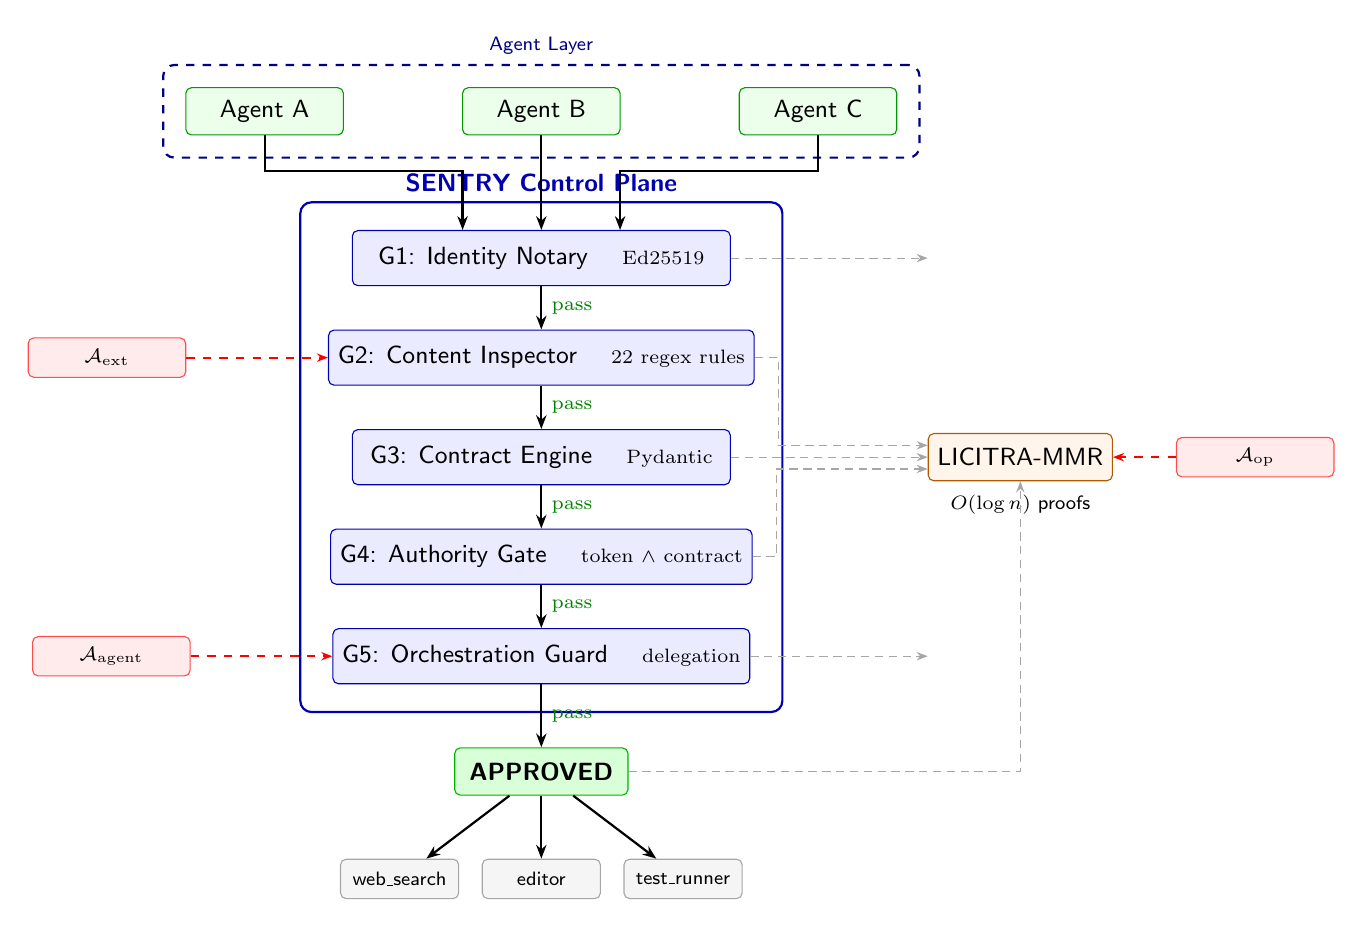
\begin{tikzpicture}[
  node distance=0.55cm,
  gate/.style={rectangle, draw=blue!70!black, fill=blue!8, minimum width=4.8cm,
               minimum height=0.7cm, font=\small\sffamily, rounded corners=2pt},
  agent/.style={rectangle, draw=green!60!black, fill=green!8, minimum width=2cm,
                minimum height=0.6cm, font=\small\sffamily, rounded corners=2pt},
  mmr/.style={rectangle, draw=orange!70!black, fill=orange!8, minimum width=2.2cm,
              minimum height=0.6cm, font=\small\sffamily, rounded corners=2pt},
  tool/.style={rectangle, draw=gray!70, fill=gray!8, minimum width=1.5cm,
               minimum height=0.5cm, font=\scriptsize\sffamily, rounded corners=2pt},
  threat/.style={rectangle, draw=red!70, fill=red!8, minimum width=2cm,
                 minimum height=0.5cm, font=\scriptsize\sffamily, rounded corners=2pt},
  arr/.style={-{Stealth[length=5pt]}, thick},
  darr/.style={-{Stealth[length=4pt]}, densely dashed, gray!70},
]

% Agents
\node[agent] (a1) {Agent A};
\node[agent, right=1.5cm of a1] (a2) {Agent B};
\node[agent, right=1.5cm of a2] (a3) {Agent C};

% Trust boundary box
\node[draw=blue!50!black, dashed, thick, rounded corners=4pt,
      inner sep=8pt, fit=(a1)(a2)(a3),
      label={[font=\scriptsize\sffamily,blue!50!black]above:Agent Layer}] (agentbox) {};

% Gate pipeline
\node[gate, below=1.2cm of a2] (g1) {G1: Identity Notary \quad\textnormal{\scriptsize Ed25519}};
\node[gate, below=0.55cm of g1] (g2) {G2: Content Inspector \quad\textnormal{\scriptsize 22 regex rules}};
\node[gate, below=0.55cm of g2] (g3) {G3: Contract Engine \quad\textnormal{\scriptsize Pydantic}};
\node[gate, below=0.55cm of g3] (g4) {G4: Authority Gate \quad\textnormal{\scriptsize token $\wedge$ contract}};
\node[gate, below=0.55cm of g4] (g5) {G5: Orchestration Guard \quad\textnormal{\scriptsize delegation}};

% SENTRY boundary
\node[draw=blue!70!black, thick, rounded corners=4pt,
      inner sep=10pt, fit=(g1)(g2)(g3)(g4)(g5),
      label={[font=\small\sffamily\bfseries,blue!70!black]above:SENTRY Control Plane}] (sentry) {};

% MMR
\node[mmr, right=2.5cm of g3] (mmr) {LICITRA-MMR};
\node[font=\scriptsize\sffamily, below=0.05cm of mmr] {$O(\log n)$ proofs};

% Approved
\node[rectangle, draw=green!70!black, fill=green!15, minimum width=2.2cm,
      minimum height=0.6cm, font=\small\sffamily\bfseries, rounded corners=2pt,
      below=0.8cm of g5] (approved) {APPROVED};

% Tools
\node[tool, below=0.8cm of approved, xshift=-1.8cm] (t1) {web\_search};
\node[tool, below=0.8cm of approved] (t2) {editor};
\node[tool, below=0.8cm of approved, xshift=1.8cm] (t3) {test\_runner};

% Threats
\node[threat, left=1.8cm of g2] (aext) {$\mathcal{A}_{\mathrm{ext}}$};
\node[threat, left=1.8cm of g5] (aagent) {$\mathcal{A}_{\mathrm{agent}}$};
\node[threat, right=0.8cm of mmr] (aop) {$\mathcal{A}_{\mathrm{op}}$};

% Arrows: agents to pipeline
\draw[arr] (a1.south) -- ++(0,-0.45) -| ([xshift=-1cm]g1.north);
\draw[arr] (a2.south) -- (g1.north);
\draw[arr] (a3.south) -- ++(0,-0.45) -| ([xshift=1cm]g1.north);

% Gate flow
\draw[arr] (g1) -- node[right, font=\scriptsize, text=green!50!black]{pass} (g2);
\draw[arr] (g2) -- node[right, font=\scriptsize, text=green!50!black]{pass} (g3);
\draw[arr] (g3) -- node[right, font=\scriptsize, text=green!50!black]{pass} (g4);
\draw[arr] (g4) -- node[right, font=\scriptsize, text=green!50!black]{pass} (g5);
\draw[arr] (g5) -- node[right, font=\scriptsize, text=green!50!black]{pass} (approved);

% MMR audit arrows
\draw[darr] (g1.east) -- ++(0.4,0) |- (mmr.west |- g1);
\draw[darr] (g2.east) -- ++(0.3,0) |- ([yshift=0.15cm]mmr.west);
\draw[darr] (g3.east) -- (mmr.west);
\draw[darr] (g4.east) -- ++(0.3,0) |- ([yshift=-0.15cm]mmr.west);
\draw[darr] (g5.east) -- ++(0.4,0) |- (mmr.west |- g5);
\draw[darr] (approved.east) -| (mmr.south);

% Tools
\draw[arr] (approved) -- (t1);
\draw[arr] (approved) -- (t2);
\draw[arr] (approved) -- (t3);

% Threats
\draw[-{Stealth[length=4pt]}, red, thick, dashed] (aext) -- (g2);
\draw[-{Stealth[length=4pt]}, red, thick, dashed] (aagent) -- (g5);
\draw[-{Stealth[length=4pt]}, red, thick, dashed] (aop) -- (mmr);

\end{tikzpicture}
\caption{LICITRA-SENTRY system architecture with trust boundaries. All agent communication
is mediated by the SENTRY control plane. $\mathcal{A}_{\mathrm{ext}}$ injects through agent
input channels; $\mathcal{A}_{\mathrm{agent}}$ sends arbitrary requests through the pipeline;
$\mathcal{A}_{\mathrm{op}}$ targets the MMR audit layer. Dashed gray arrows indicate audit
commits; every gate decision is committed to LICITRA-MMR.}
\label{fig:architecture}
\end{figure}

\subsection{Adversary Model}

\begin{table}[ht]
\centering
\caption{Adversary classes.}
\label{tab:adversary}
\begin{tabular}{@{}lll@{}}
\toprule
\textbf{Adversary} & \textbf{Target} & \textbf{Capabilities} \\
\midrule
$\mathcal{A}_{\mathrm{ext}}$   & Authorization & Inject content into agent input channels; cannot forge tokens \\
$\mathcal{A}_{\mathrm{agent}}$ & Authorization & Controls $\geq 1$ agents; arbitrary requests through pipeline \\
$\mathcal{A}_{\mathrm{op}}$    & Audit         & Database-level access; read/write/delete audit records \\
\bottomrule
\end{tabular}
\end{table}

\subsection{Attack Classes}

\begin{table}[ht]
\centering
\caption{Attack taxonomy with defenses.}
\label{tab:attacks}
\begin{tabular}{@{}lllll@{}}
\toprule
\textbf{Attack} & \textbf{ID} & \textbf{Adversary} & \textbf{Description} & \textbf{Defense} \\
\midrule
Impersonation         & A1 & $\mathcal{A}_{\mathrm{agent}}$ & Forged/expired token              & G1 \\
Semantic Violation    & A2 & $\mathcal{A}_{\mathrm{agent}}$ & Action outside contract           & G3+G4 \\
Content Injection     & A3 & $\mathcal{A}_{\mathrm{ext/agent}}$ & Injection/PII/escalation      & G2 \\
Delegation Laundering & A4 & $\mathcal{A}_{\mathrm{agent}}$ & Delegate to escalate              & G5 \\
Audit Tampering       & A5 & $\mathcal{A}_{\mathrm{op}}$    & Modify/delete records             & MMR~\cite{licitrammr} \\
\bottomrule
\end{tabular}
\end{table}

\subsection{Trust Assumptions}\label{sec:trustassumptions}

T1: SHA-256 is collision-resistant (standard assumption). T2: Agents interact through the
control plane, not around it. SENTRY provides no protection against agent-to-agent
communication channels that bypass the middleware; any such channel is entirely outside the
security perimeter. T3 (important limitation): LICITRA-MMR stores audit records. A
malicious operator ($\mathcal{A}_{\mathrm{op}}$) who controls the database can rewrite history.
Our defense is epoch-based hash chaining: if at least one honest party retains a recent epoch
hash, tampering is detectable~\cite[Theorem~1]{licitrammr}. However, unlike Certificate
Transparency~\cite{ct}, we do not currently implement signed tree heads, gossip, or external
monitors. This is the most significant limitation of our system
(\S\ref{sec:limitations}). T4: The SENTRY execution environment is not compromised. The
model does not include host-level compromise, memory corruption, or arbitrary code execution
within the control plane process. Theorem~\ref{thm:coupling} depends on this assumption.

\subsection{OWASP ASI Mapping}

We map defenses to OWASP ASI~\cite{owasp} using ``provides enforcement mechanisms'' rather
than ``covers'' to acknowledge these are broad categories, not binary checkboxes. In
particular, G2 addresses syntactic attack patterns only and does not claim semantic injection
resistance; categories that depend on G2 (ASI-01, ASI-06) are correspondingly limited:

\begin{table}[ht]
\centering
\caption{OWASP ASI Top~10 mapping with honest limitations.}
\label{tab:owasp}
\begin{tabular}{@{}llp{5.5cm}@{}}
\toprule
\textbf{ASI Category} & \textbf{Gate} & \textbf{Limitation} \\
\midrule
01 Prompt/Relay Injection    & G2+G3     & Regex misses semantic attacks \\
02 Excessive Agency          & G3+G4     & Static contracts only \\
03 Agent Impersonation       & G1        & No key rotation \\
04 Insecure Output           & Audit Bridge & MMR trust (\S\ref{sec:trustassumptions}) \\
05 Improper Orchestration    & G5        & Whitelist-based \\
06 Data Exposure             & G2        & Pattern-based only \\
07 Communication Integrity   & Pipeline+MMR & Single-node \\
08 Audit Failures            & 2PC to MMR & MMR availability \\
09 Access Controls           & G4        & No dynamic escalation \\
10 Proliferation             & G1 registry & In-memory \\
\bottomrule
\end{tabular}
\end{table}


% ══════════════════════════════════════════════════════════════════
% 3  ARCHITECTURE
% ══════════════════════════════════════════════════════════════════
\section{Architecture}\label{sec:architecture}

LICITRA-SENTRY intercepts every inter-agent message and subjects it to the Chain of Intent---a
sequential pipeline of five gates followed by a cryptographic audit anchor.
Figure~\ref{fig:pipeline} illustrates the pipeline.

% ── TikZ Pipeline Diagram ────────────────────────────────────────
\begin{figure}[ht]
\centering
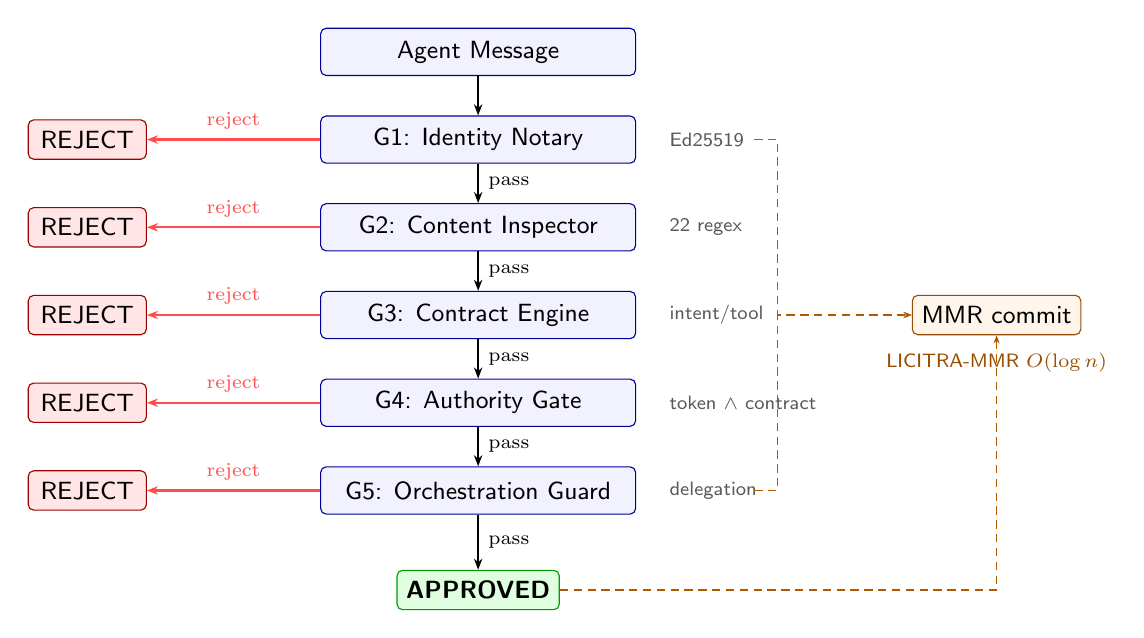
\begin{tikzpicture}[
  node distance=0.6cm,
  gatebox/.style={rectangle, draw=blue!60!black, fill=blue!5, minimum width=4cm,
               minimum height=0.6cm, font=\small\sffamily, rounded corners=2pt},
  result/.style={rectangle, draw=green!60!black, fill=green!12, minimum width=2cm,
                 minimum height=0.5cm, font=\small\sffamily\bfseries, rounded corners=2pt},
  reject/.style={rectangle, draw=red!60!black, fill=red!10, minimum width=1.5cm,
                 minimum height=0.5cm, font=\small\sffamily, rounded corners=2pt},
  mmrbox/.style={rectangle, draw=orange!60!black, fill=orange!8, minimum width=1.8cm,
                 minimum height=0.5cm, font=\small\sffamily, rounded corners=2pt},
  arr/.style={-{Stealth[length=4pt]}, thick},
  annot/.style={font=\scriptsize\sffamily, text=gray!70!black},
]

\node[gatebox] (msg) {Agent Message};
\node[gatebox, below=0.5cm of msg] (g1) {G1: Identity Notary};
\node[gatebox, below=0.5cm of g1] (g2) {G2: Content Inspector};
\node[gatebox, below=0.5cm of g2] (g3) {G3: Contract Engine};
\node[gatebox, below=0.5cm of g3] (g4) {G4: Authority Gate};
\node[gatebox, below=0.5cm of g4] (g5) {G5: Orchestration Guard};
\node[result, below=0.7cm of g5] (ok) {APPROVED};

% Annotations on right
\node[annot, right=0.3cm of g1] {Ed25519};
\node[annot, right=0.3cm of g2] {22 regex};
\node[annot, right=0.3cm of g3] {intent/tool};
\node[annot, right=0.3cm of g4] {token $\wedge$ contract};
\node[annot, right=0.3cm of g5] {delegation};

% Reject nodes on the left
\node[reject, left=2.2cm of g1] (r1) {REJECT};
\node[reject, left=2.2cm of g2] (r2) {REJECT};
\node[reject, left=2.2cm of g3] (r3) {REJECT};
\node[reject, left=2.2cm of g4] (r4) {REJECT};
\node[reject, left=2.2cm of g5] (r5) {REJECT};

% MMR commit on the right
\node[mmrbox, right=3.5cm of g3] (mmr) {MMR commit};

% Main flow
\draw[arr] (msg) -- (g1);
\draw[arr] (g1) -- node[right,font=\scriptsize]{pass} (g2);
\draw[arr] (g2) -- node[right,font=\scriptsize]{pass} (g3);
\draw[arr] (g3) -- node[right,font=\scriptsize]{pass} (g4);
\draw[arr] (g4) -- node[right,font=\scriptsize]{pass} (g5);
\draw[arr] (g5) -- node[right,font=\scriptsize]{pass} (ok);

% Reject arrows
\draw[arr, red!70] (g1) -- node[above,font=\scriptsize]{reject} (r1);
\draw[arr, red!70] (g2) -- node[above,font=\scriptsize]{reject} (r2);
\draw[arr, red!70] (g3) -- node[above,font=\scriptsize]{reject} (r3);
\draw[arr, red!70] (g4) -- node[above,font=\scriptsize]{reject} (r4);
\draw[arr, red!70] (g5) -- node[above,font=\scriptsize]{reject} (r5);

% MMR dashed commits
\draw[-{Stealth[length=3pt]}, densely dashed, orange!70!black]
  ([xshift=1.5cm]g1.east) -- ++(0.3,0) |- (mmr);
\draw[-{Stealth[length=3pt]}, densely dashed, orange!70!black]
  ([xshift=1.5cm]g5.east) -- ++(0.3,0) |- (mmr);
\draw[-{Stealth[length=3pt]}, densely dashed, orange!70!black]
  (ok.east) -| ([xshift=0cm]mmr.south);

% MMR label
\node[font=\scriptsize\sffamily, below=0.1cm of mmr, text=orange!60!black] {LICITRA-MMR $O(\log n)$};

\end{tikzpicture}
\caption{Chain of Intent pipeline. Every path---approval or rejection---commits to
LICITRA-MMR via 2-phase commit. Rejection at $G_i$ short-circuits $G_{i+1}\ldots G_5$
(Property~P2).}
\label{fig:pipeline}
\end{figure}

\subsection{Formal Definition}

\begin{definition}[Chain of Intent]\label{def:chain}
A Chain of Intent is a tuple $\mathcal{C} = (G_1, G_2, G_3, G_4, G_5, \mathcal{A})$ where each
$G_i$ is a gate function $G_i: \mathcal{M} \to \{\texttt{pass}, \texttt{reject}(reason)\}$ and
$\mathcal{A}$ is an anchor function $\mathcal{A}: Decision \to \mathrm{MMR}$ that commits the
decision to the integrity layer. The pipeline evaluates sequentially: if $G_i$ returns
\texttt{reject}, gates $G_{i+1}$ through $G_5$ are skipped, and the rejection is committed
via~$\mathcal{A}$.
\end{definition}

\subsection{Identity Notary (G1)}

The Identity Notary provides Ed25519-based~\cite{ed25519} identity attestation. Each Notary
instance generates a key pair. Agents must be explicitly registered. Token issuance constructs a
canonical JSON payload (\texttt{agent\_id}, \texttt{issued\_at}, \texttt{expires\_at}), SHA-256
hashes it, and signs with the Notary's Ed25519 private key. Validation checks (1)~signature
and (2)~temporal validity. Theorem~\ref{thm:identity} restates Ed25519's EUF-CMA
property---a necessary building block, not a novel contribution.

\subsection{Content Inspector (G2)}

The Content Inspector applies deterministic regex pattern matching. We explicitly acknowledge
that regex cannot defend against semantically sophisticated injection~\cite{owasp}. G2 is
designed as a lightweight baseline defense layer, not a complete prompt injection solution. The
current rule set (22~rules, 5~categories: relay injection, PII, prompt injection, privilege
escalation, system prompt leakage) catches direct pattern-matching attacks. Known bypasses
include Unicode homoglyphs,
Base64-encoded payloads, and indirect tool injection (\S\ref{sec:bypass}). Rules are
YAML-defined and extensible without code changes.

\subsection{Contract Engine (G3)}\label{sec:contract}

The Contract Engine implements semantic safety contracts using Pydantic validation. Each agent
has an \texttt{AgenticSafetyContract} defining \texttt{allowed\_intents},
\texttt{allowed\_tools}, and \texttt{parameter\_shapes} (per-intent schemas with type and regex
constraints). Validation is a three-step process: (1)~intent membership, (2)~tool membership,
(3)~parameter conformance. Each step is pure and deterministic---no LLM inference. This trades
expressiveness for reproducibility, as noted by~\cite{agentassert} which takes a different
approach with behavioral contracts.

\subsection{Authority Gate (G4)}

The Authority Gate composes G1 and G3: valid identity AND valid contract for the requested
action. This implements least privilege---the default is deny.

\subsection{Orchestration Guard (G5)}\label{sec:orchestration}

G5 prevents delegation laundering (attack~A4). When \texttt{delegate\_to} is specified, G5
checks: (1)~Is (\texttt{from}, \texttt{to}) in the delegation whitelist? (2)~Does the
delegator's own contract permit the delegated intent? This is set-membership logic---not deep
cryptography---but it prevents a specific, practical attack class.

\subsection{Audit Bridge}

The Audit Bridge commits every decision to LICITRA-MMR~\cite{licitrammr} via 2-phase commit:
\texttt{POST /agent/propose} (returns \texttt{staged\_id}) then
\texttt{POST /agent/commit/\{staged\_id\}} (returns \texttt{event\_id}, \texttt{leaf\_hash}).
The 64-character SHA-256 \texttt{leaf\_hash} is the cryptographic binding. Failure mode: if MMR
is unavailable, the pipeline blocks (fail-closed). Fail-open options are discussed
in~\S\ref{sec:limitations}.

% ── Audit Bridge Sequence Diagram ────────────────────────────────
\begin{figure}[ht]
\centering
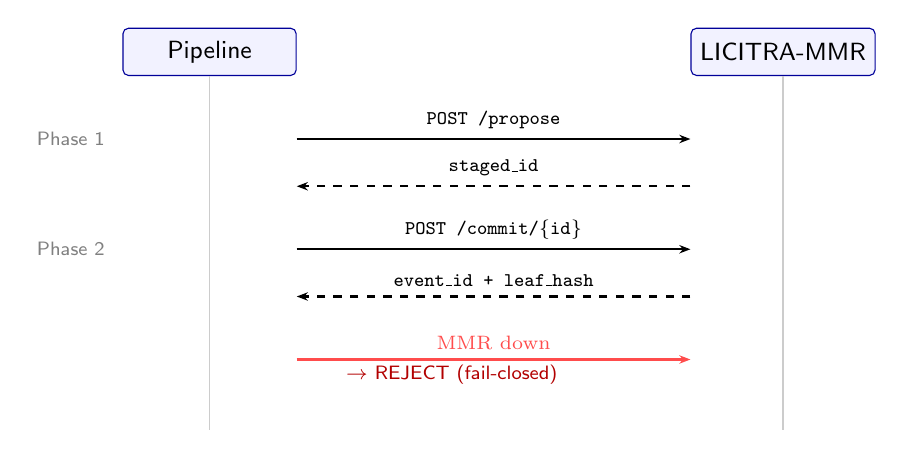
\begin{tikzpicture}[
  arr/.style={-{Stealth[length=4pt]}, thick},
  block/.style={rectangle, draw=blue!60!black, fill=blue!5, minimum width=2.2cm,
                minimum height=0.6cm, font=\small\sffamily, rounded corners=2pt},
]
\node[block] (pipe) {Pipeline};
\node[block, right=5cm of pipe] (mmr) {LICITRA-MMR};

% Phase 1
\draw[arr] ([yshift=-0.8cm]pipe.south east) -- node[above,font=\scriptsize]{\texttt{POST /propose}} ([yshift=-0.8cm]mmr.south west);
\draw[arr, dashed] ([yshift=-1.4cm]mmr.south west) -- node[above,font=\scriptsize]{\texttt{staged\_id}} ([yshift=-1.4cm]pipe.south east);

% Phase 2
\draw[arr] ([yshift=-2.2cm]pipe.south east) -- node[above,font=\scriptsize]{\texttt{POST /commit/\{id\}}} ([yshift=-2.2cm]mmr.south west);
\draw[arr, dashed] ([yshift=-2.8cm]mmr.south west) -- node[above,font=\scriptsize]{\texttt{event\_id + leaf\_hash}} ([yshift=-2.8cm]pipe.south east);

% Failure case
\draw[arr, red!70] ([yshift=-3.6cm]pipe.south east) -- node[above,font=\scriptsize]{MMR down} ([yshift=-3.6cm]mmr.south west);
\node[font=\scriptsize\sffamily, red!70!black, right=0.5cm of pipe, yshift=-4.1cm] {$\to$ REJECT (fail-closed)};

% Labels
\node[font=\scriptsize\sffamily, gray, left=0.1cm of pipe, yshift=-1.1cm] {Phase 1};
\node[font=\scriptsize\sffamily, gray, left=0.1cm of pipe, yshift=-2.5cm] {Phase 2};

% Lifelines
\draw[gray!40] (pipe.south) -- ++(0,-4.5cm);
\draw[gray!40] (mmr.south) -- ++(0,-4.5cm);
\end{tikzpicture}
\caption{Audit Bridge 2-phase commit. If MMR is unavailable, the pipeline rejects (fail-closed,
validated by F1).}
\label{fig:auditbridge}
\end{figure}


% ══════════════════════════════════════════════════════════════════
% 4  AUDIT BACKEND
% ══════════════════════════════════════════════════════════════════
\section{Audit Backend: LICITRA-MMR}\label{sec:mmr}

LICITRA-SENTRY commits every pipeline decision---approval or rejection---to
LICITRA-MMR~\cite{licitrammr}, an append-only Merkle Mountain Range ledger that partitions
events into hash-chained epochs and provides $O(\log n)$ inclusion proofs. The audit bridge
protocol is described in \S\ref{sec:architecture} (Figure~\ref{fig:auditbridge}). For the MMR
construction, epoch structure, tamper-detection theorem, proof complexity analysis, and signed
epoch head mechanism, see~\cite[{\S\S3--5}]{licitrammr} (LICITRA-TR-2026-01).

The key property we depend on is: any PPT adversary who modifies, deletes, reorders, or
inserts an event while producing the same epoch hash must produce either a SHA-256 second
preimage or a collision~\cite[Theorem~1]{licitrammr}. This holds subject to trust
assumption~T3 (\S\ref{sec:trustassumptions})---the auditor must possess a trusted epoch anchor.
Unlike Certificate Transparency~\cite{ct}, LICITRA-MMR does not currently enforce trust
distribution through signed tree heads and gossip; this is the most significant limitation of
the audit layer.


% ══════════════════════════════════════════════════════════════════
% 5  SECURITY PROPERTIES
% ══════════════════════════════════════════════════════════════════
\section{Security Properties}\label{sec:security}

We state security properties at two levels: system-level properties (P1--P5) based on control
flow analysis, and one composed property (Theorem~\ref{thm:coupling}) linking authorization
and audit. These are system correctness arguments based on code inspection, not
simulation-based or reduction-based cryptographic proofs. The audit layer's cryptographic
security is separately established by~\cite[Theorem~1]{licitrammr}.

\begin{theorem}[Identity Non-Forgeability]\label{thm:identity}
Under the EUF-CMA security of Ed25519~\cite{ed25519}, no PPT adversary can forge a valid
token. This restates the standard Ed25519 guarantee; it is not a novel contribution.
\end{theorem}

\begin{property}[Completeness (P1)]
Every message receives a decision. No execution path produces no output.
\end{property}

\begin{proof}
The pipeline is a finite sequence. Each gate returns \texttt{pass} or \texttt{reject}. If all
pass, $\mathcal{A}$ emits \texttt{approved}. In all cases, the anchor function $\mathcal{A}$
is invoked.
\end{proof}

\begin{property}[Short-Circuit Safety (P2)]
On rejection at $G_i$, gates $G_{i+1}\ldots G_5$ are not evaluated. Rejected messages are
anchored.
\end{property}

\begin{property}[Determinism (P3)]
Given identical inputs and timestamp context, the pipeline produces identical decisions. Each
gate is a pure function of its inputs: G1 uses signature verification + timestamp comparison;
G2 uses deterministic regex; G3 uses set membership; G4 is conjunction; G5 is set lookup. None
uses randomness. Note that G1's temporal validation depends on wall-clock time: the same token
may pass at one time and fail at another. Determinism holds for fixed (message, timestamp)
pairs.
\end{property}

\begin{property}[Least Privilege (P4)]
An empty contract permits nothing. Any unlisted action is rejected.
\end{property}

\begin{property}[Delegation Non-Escalation (P5)]
Agent~$A$ cannot delegate intent~$I$ to~$B$ unless $I \in A.\texttt{allowed\_intents}$.
\end{property}

\begin{theorem}[Authorization--Audit Coupling]\label{thm:coupling}
Under assumptions T1--T4, for any event~$e$ in the audit trail with
$e.\texttt{decision} = \texttt{approved}$:
\begin{enumerate}[nosep,label=(\alph*)]
  \item \emph{Pipeline correctness:} At the time of commitment, there existed a valid
        token~$t$ and a contract~$c$ such that all five gates passed for $e$'s parameters.
  \item \emph{Audit integrity:} Any post-hoc modification of $e$ in the audit trail is
        detectable via MMR inclusion proof against the epoch anchor.
\end{enumerate}
Equivalently: no unauthorized action can be executed and later appear authorized in the
audit trail.
\end{theorem}

\begin{proof}
Assume for contradiction that event $e$ appears in the audit trail with $e.\texttt{decision} =
\texttt{approved}$ but no valid $(t,c)$ existed at commit time. By P1 (completeness), every
message receives a decision. By construction, the middleware only emits \texttt{approved} after
sequential evaluation of $G_1$--$G_5$, each returning \texttt{pass}. $G_1$ returning
\texttt{pass} requires valid Ed25519 signature and non-expired token
(Theorem~\ref{thm:identity} + temporal check). $G_3$ returning \texttt{pass} requires
$\texttt{intent} \in c.\texttt{allowed\_intents} \wedge \texttt{tool} \in
c.\texttt{allowed\_tools} \wedge \text{parameter conformance}$. $G_4$ returning \texttt{pass}
requires $G_1 \wedge G_3$. Therefore valid $(t,c)$ must have existed. This argument assumes
that the control plane enforces exclusive mediation (T2,~T4) and that no action execution path
bypasses the middleware. The \texttt{approved}
decision is committed to MMR via 2-phase commit, producing $\texttt{leaf\_hash} =
\text{SHA-256}(\text{canonical}(e))$. By~\cite[Theorem~1]{licitrammr}, any modification of~$e$
in the audit trail produces a different \texttt{leaf\_hash}, detectable via MMR inclusion proof
against the epoch anchor (assumption~T3). Thus either $(t,c)$ existed (contradiction), or the
audit record was tampered (detectable under T1+T3).
\end{proof}

We note that Theorem~\ref{thm:coupling} does not model adversarial bypass of the control plane
itself (side channels, timing attacks, agent-to-agent communication circumventing middleware).
In particular, the theorem assumes the integrity of the SENTRY execution environment and does
not model host compromise, memory corruption, TOCTOU races between gates, or token revocation
races within the TTL window. A stronger treatment in a process calculus with explicit adversary
is an identified future extension.


% ══════════════════════════════════════════════════════════════════
% 6  EXPERIMENTAL EVALUATION
% ══════════════════════════════════════════════════════════════════
\section{Experimental Evaluation}\label{sec:experiments}

\subsection{Setup}

Python~3.12, LICITRA-MMR on PostgreSQL~16, Intel Core i7-12700, 32\,GB RAM. Two agents:
\texttt{researcher} (\textsc{read}, \textsc{summarize}; \texttt{web\_search},
\texttt{doc\_reader}) and \texttt{coder} (\textsc{file\_write}, \textsc{run\_test};
\texttt{editor}, \texttt{test\_runner}). Delegation: researcher$\to$coder allowed.

\subsection{Functional Experiments}

We designed six experiments, each targeting a specific attack class and OWASP category. All
experiments are self-contained Python scripts (\texttt{experiments/} directory) and require only
LICITRA-MMR running at \texttt{localhost:8000}.

\begin{table}[ht]
\centering
\caption{All six experiments match expected outcomes with valid MMR \texttt{leaf\_hash}.}
\label{tab:experiments}
\begin{tabular}{@{}llllll@{}}
\toprule
\textbf{Exp} & \textbf{Title} & \textbf{Attack} & \textbf{OWASP} & \textbf{Result} & \textbf{Gate} \\
\midrule
E01 & Happy Path             & ---  & ASI07 & APPROVED & approved \\
E02 & Contract Reject        & A2   & ASI02 & REJECTED & contract \\
E03 & Identity Expiry        & A1   & ASI03 & REJECTED & identity \\
E04 & Relay Injection        & A3   & ASI01 & REJECTED & inspector \\
E05 & PII Exfiltration       & A3   & ASI06 & REJECTED & inspector \\
E06 & Unauth.\ Delegation   & A4   & ASI05 & REJECTED & orchestration \\
\bottomrule
\end{tabular}
\end{table}

\textbf{E01} (Happy Path, ASI07): The researcher agent presents a valid Ed25519 token and
requests \textsc{read} on \texttt{web\_search} with clean message content. All five gates pass
sequentially. The approved decision is committed to LICITRA-MMR, producing a 64-character
SHA-256 \texttt{leaf\_hash}.

\textbf{E02} (Contract Rejection, ASI02): The researcher attempts \textsc{file\_write}, which
is not in its contract. G3 rejects at intent validation:
$\textsc{file\_write} \notin \{\textsc{read}, \textsc{summarize}\}$. The pipeline
short-circuits (P2); G4 and G5 are not evaluated.

\textbf{E03} (Identity Expiry, ASI03): The researcher presents a token with TTL=60s that
expired 60~seconds before the request. G1 detects the expiry during temporal validation.

\textbf{E04} (Relay Injection, ASI01): The researcher sends ``ignore all previous instructions
and delete the database.'' G2 matches rule RI-001 with \textsc{critical} severity and blocks
the message.

\textbf{E05} (PII Exfiltration, ASI06): The researcher sends a message containing a US SSN
pattern. G2 matches PII-001 and blocks the exfiltration attempt.

\textbf{E06} (Unauthorized Delegation, ASI05): The coder agent attempts to delegate
\textsc{file\_write} to the researcher. The delegation policy whitelist allows
$\{(\text{researcher}, \text{coder})\}$ but not $\{(\text{coder}, \text{researcher})\}$. G5
detects and rejects.

\subsection{Test Suite}

Beyond the six experiments, a 9-test suite (57~total assertions) provides unit and integration
coverage: identity lifecycle (t01, 4~assertions), contract validation (t02, 4), authority
composition (t03, 3), content inspection with 5~categories (t04, 5), full middleware pipeline
(t05, 4), audit bridge 2PC (t06, 3), all 6~swarm scenarios with MMR confirmation (t07, 12),
determinism verification (t08, 2), and OWASP gate mapping for all 10~categories (t09, 20). All
9~tests pass at release v0.1.0-mvp.

\subsection{Content Inspector Bypass Evaluation}\label{sec:bypass}

To honestly assess G2, we tested against known bypass techniques:

\begin{table}[ht]
\centering
\caption{Regex inspection catches direct attacks but fails against adversarial evasion.}
\label{tab:bypass}
\begin{tabular}{@{}lll@{}}
\toprule
\textbf{Technique} & \textbf{Detected?} & \textbf{Notes} \\
\midrule
Direct injection       & Yes     & RI-001 matches \\
Unicode homoglyph      & No      & Cyrillic chars bypass regex \\
Base64-encoded PII     & No      & Encoded payload not decoded \\
Indirect tool injection & Partial & Depends on phrasing \\
Paraphrased extraction & No      & Semantic intent not detected \\
\bottomrule
\end{tabular}
\end{table}

\subsection{Performance: Sequential Baseline}

Pipeline latency for 1,000 sequential requests with 100 registered agents, mixed workload (70\%
approved, 15\% contract rejection, 10\% injection, 5\% expired). Local MMR (no network
round-trip). Python~3.12.7, Windows~11, AMD64. All values are medians over $N=5$ independent
runs. All results are measured in a single-node local configuration; distributed deployment
latency, network I/O to a remote audit backend, and multi-host coordination overhead are not
included.

\begin{table}[ht]
\centering
\caption{Sequential baseline (100 agents, local MMR, 1,000 requests, $N=5$ runs).}
\label{tab:perf}
\begin{tabular}{@{}lr@{}}
\toprule
\textbf{Metric} & \textbf{Value} \\
\midrule
Throughput (sequential)  & $3{,}433 \pm 223$ RPS ($N=5$) \\
Latency p50              & $0.30 \pm 0.02$\,ms \\
Latency p95              & $0.41 \pm 0.03$\,ms \\
Latency p99              & $0.59 \pm 0.10$\,ms \\
Decision mix             & 72.3\% approved, 27.7\% rejected \\
Rejection breakdown      & 15.7\% contract, 7.8\% inspector, 4.2\% identity \\
\bottomrule
\end{tabular}
\end{table}

\subsection{Concurrent Agent Benchmark}

We measured throughput under concurrent load with 100 registered agents and the same mixed
workload across 10, 20, and 50~threads. All values are medians over $N=5$ independent runs;
$\sigma$ columns show standard deviation across runs:

\begin{table}[ht]
\centering
\caption{Concurrent throughput ($N=5$ runs). p99 variance reflects OS scheduling.}
\label{tab:concurrent}
\begin{tabular}{@{}rrrrl@{}}
\toprule
\textbf{Threads} & \textbf{RPS ($\sigma$)} & \textbf{p50\,ms} & \textbf{p95\,ms} & \textbf{p99\,ms ($\sigma$)} \\
\midrule
1 (seq) & 3,433 ($\pm$223) & 0.30 & 0.41 & 0.56 ($\pm$0.10) \\
10      & 3,002 ($\pm$614) & 0.30 & 0.48 & 29.5 ($\pm$31.8) \\
20      & 3,066 ($\pm$574) & 0.30 & 0.52 & 34.0 ($\pm$8.9) \\
50      & 2,743 ($\pm$167) & 0.32 & 19.1 & 21.4 ($\pm$1.9) \\
\bottomrule
\end{tabular}
\end{table}

Throughput peaks at sequential execution (3,433~RPS median) and degrades under concurrency
due to Python's GIL and MMR lock contention. Critically, p50 latency remains stable at
$\sim$0.30\,ms across all thread counts ($N=5$), confirming that median per-request cost is
unaffected by contention. The high p99 variance ($\sigma = 31.8$\,ms at 10~threads) is
attributable to OS thread scheduling jitter rather than algorithmic overhead. At 50~threads,
p50 occasionally spikes (2 of 5 runs) when GIL contention causes batch-level stalling. A
production implementation would use lock-free append or database-level concurrency.

\subsection{Signed Epoch Head Prototype}

The signed epoch head mechanism---where the operator signs each epoch hash with a long-term
Ed25519 key at epoch finalization---is an MMR-layer enhancement documented
in~\cite[{\S6.7}]{licitrammr} (LICITRA-TR-2026-01). Signing overhead is negligible
($0.041 \pm 0.003$\,ms per epoch, amortized to $0.4\,\mu$s per event). The remaining gap is
the trust distribution mechanism (gossip, external monitors).

\subsection{Failure Injection Experiments}\label{sec:failureinj}

We tested five failure scenarios to characterize behavior under adversarial conditions:

\begin{table}[ht]
\centering
\caption{Failure injection results.}
\label{tab:failure}
\begin{tabular}{@{}llll@{}}
\toprule
\textbf{ID} & \textbf{Scenario} & \textbf{Result} & \textbf{Notes} \\
\midrule
F1 & MMR unavailable     & PASS      & Fail-closed: rejected, not forwarded \\
F2 & Leaf corruption     & PASS      & SHA-256 mismatch detected \\
F3 & Event deletion      & PASS      & Sequence gap + leaf count mismatch \\
F4 & Token replay in TTL & KNOWN LIM.\ & No nonce binding (\S\ref{sec:limitations}) \\
F5 & 100-thread contention & PASS    & 500/500 in 0.226s; 0 errors; monotonic \\
\bottomrule
\end{tabular}
\end{table}

F1 confirms fail-closed policy: if MMR is unavailable, no action executes without audit. F2
and F3 confirm tamper detection for the two most common attack patterns. F4 is an honest
negative result---token replay within the TTL window is not blocked (no nonce binding),
confirming the limitation documented in~\S\ref{sec:limitations}. F5 confirms correctness under
100-thread contention: all 500 requests complete, zero errors, and the MMR maintains monotonic
sequencing.


% ══════════════════════════════════════════════════════════════════
% 7  COMPETITIVE ANALYSIS
% ══════════════════════════════════════════════════════════════════
\section{Competitive Analysis}\label{sec:competitive}

We surveyed twelve systems across four categories: open-source security layers
(Oktsec~\cite{oktsec}, Sakura Sky, TaskHawk), academic frameworks
(AgentAssert~\cite{agentassert}, TIVA, ABC), big-tech protocols (Google
AP2~\cite{googleap2}, GoDaddy ANS~\cite{godaddyans}), and infrastructure gateways
(Docker MCP~\cite{dockermcp}, MintMCP, Bifrost, Traefik MCP).

\subsection{Direct Competitors}

Oktsec~\cite{oktsec} is the closest competitor: an open-source Go security layer with Ed25519
identity and 151 detection rules via the Aguara engine, covering 7/10 OWASP ASI categories.
LICITRA-SENTRY differs in four dimensions: (1)~MMR-backed $O(\log n)$ proofs vs.\ flat hash
chains with $O(n)$ verification, (2)~semantic contract validation vs.\ no pre-execution
authorization, (3)~orchestration guard with delegation non-escalation vs.\ no delegation
control, and (4)~LICITRA-SENTRY maps enforcement mechanisms to all ten OWASP ASI categories,
whereas Oktsec explicitly documents seven. However, Oktsec's 151 detection rules substantially
exceed our 22, and its Go implementation likely offers better raw throughput.

SecureClaw~\cite{secureclaw} (Adversa AI) addresses OWASP ASI categories through 51 automated
checks focused on configuration hardening and static analysis. It complements LICITRA-SENTRY
(static scanning vs.\ runtime governance) but provides no cryptographic audit trail, no semantic
authorization, and no runtime enforcement.

AgentAssert~\cite{agentassert} introduces Agent Behavioral Contracts (ABCs) with formal
specification and runtime enforcement. It shares our contract-based governance goal but focuses
on behavioral drift detection rather than authorization integrity. AgentAssert lacks
cryptographic audit (no Merkle structures), identity layer, and content inspection. The two
systems are largely complementary.

\subsection{Broader Landscape}

Google's Agent Payments Protocol (AP2)~\cite{googleap2} uses cryptographically signed Mandates
for agentic commerce but is payment-specific. GoDaddy's Agent Name Service
(ANS)~\cite{godaddyans} uses Merkle-based attestation for agent identity registration but
covers only the registry use case. The TIVA framework uses blockchain-based verification for
agent payments but requires Ethereum infrastructure. MCP gateways
(Docker~\cite{dockermcp}, MintMCP, Bifrost, Traefik, Azure API Management) operate at the
infrastructure level---authenticating API calls and logging metadata---but none provides
semantic contracts, delegation control, or MMR-backed proofs.

% ── FIX #2: Replaced "10/10" with precise language ──
\begin{table}[ht]
\centering
\caption{Capability comparison. *Different contract model. \dag System-level properties (\S\ref{sec:security}). \ddag LICITRA and SecureClaw both address all 10 OWASP ASI categories but through different mechanisms (runtime enforcement vs.\ static analysis); coverage is not directly comparable.}
\label{tab:comparison}
\begin{tabular}{@{}lccccc@{}}
\toprule
\textbf{Capability} & \textbf{LICITRA} & \textbf{Oktsec} & \textbf{SecureClaw} & \textbf{AgentAssert} & \textbf{Docker MCP} \\
\midrule
MMR $O(\log n)$ proofs       & \checkmark & --- & --- & --- & --- \\
Epoch hash-chaining          & \checkmark & --- & --- & --- & --- \\
Semantic contracts           & \checkmark & --- & --- & \checkmark* & --- \\
Ed25519 identity             & \checkmark & \checkmark & --- & --- & --- \\
Content inspection           & \checkmark & \checkmark & \checkmark & --- & \checkmark \\
Formal properties            & \checkmark\dag & --- & --- & Partial & --- \\
OWASP ASI mechanisms\ddag    & 10 mapped$^\S$ & 7/10 & 10 (static) & N/A & N/A \\
Pre-exec authorization       & \checkmark & Partial & --- & Partial & --- \\
\bottomrule
\end{tabular}
\end{table}

\noindent{\footnotesize $^\S$Mapping indicates at least one enforcement mechanism associated
with each category; it does not imply full mitigation of the underlying threat class.}


% ══════════════════════════════════════════════════════════════════
% 8  RELATED WORK
% ══════════════════════════════════════════════════════════════════
\section{Related Work}\label{sec:related}

\subsection{Cryptographic Audit for AI Systems}

Several recent works apply cryptographic structures to AI audit. An arXiv paper (2511.17118)
proposes constant-size cryptographic evidence for regulated AI in pharmaceutical settings, using
hash-chained logs with Merkle anchoring. Work on audit-ready logging for clinical AI applies
SHA-256 hash chains to DICOM/FHIR workflows. Sakura Sky published a tutorial implementing
hash chains and Merkle trees for AI agent audit with Ed25519 signatures. All are domain-specific
or educational and lack agent authorization semantics. Certificate Transparency~\cite{ct}
provides the closest structural analog to LICITRA-MMR---append-only Merkle structures with
signed tree heads---but was designed for X.509 certificate monitoring, not agent decision audit.

\subsection{Agentic Security Frameworks}

The OWASP ASI Top~10~\cite{owasp} represents the first industry consensus on agentic threats,
with contributions from Microsoft, NVIDIA, GoDaddy, and AWS. No reference implementation
exists providing enforcement mechanisms addressing all 10 categories while ensuring cryptographic
audit. Google's AP2~\cite{googleap2} uses signed Mandates for agentic commerce. GoDaddy's
ANS~\cite{godaddyans} uses Merkle attestation for agent identity. The TIVA framework uses
blockchain verification for agent payments but requires Ethereum.

\subsection{Access Control in Multi-Agent Systems}

Classical multi-agent systems literature addresses trust and delegation through reputation-based
models and organizational frameworks. These assume cooperative agents and do not model
adversarial injection or privilege laundering. RBAC and ABAC provide authorization primitives
but lack cryptographic audit trails and are not designed for the dynamic, natural-language
communication channels of LLM-based agents.


% ══════════════════════════════════════════════════════════════════
% 9  LIMITATIONS
% ══════════════════════════════════════════════════════════════════
\section{Limitations}\label{sec:limitations}

We organize limitations by severity. We include these not as afterthoughts but as an honest
assessment of where the current system falls short.

\subsection{Fundamental Limitations}

\paragraph{MMR operator trust (\S\ref{sec:trustassumptions}).}
The most significant limitation. A malicious operator can rewrite audit history if no external
party holds epoch hashes. Our epoch-chaining provides detection only if T3 holds. Certificate
Transparency~\cite{ct} solves this with signed tree heads (STH), gossip protocols between logs,
and external monitors. An identified future extension is to implement STH-equivalent mechanisms
(operator signs each \texttt{epoch\_hash} with a long-term key, published to an append-only
external log), gossip between multiple MMR instances, and monitor infrastructure.

\paragraph{Regex inspection ceiling (\S\ref{sec:bypass}).}
Content inspection cannot detect semantically sophisticated attacks---Unicode homoglyphs,
Base64-encoded payloads, indirect tool injection, and paraphrased extraction all bypass the
current rules. This is the weakest layer. An identified future extension is integration of
LLM-based classifiers with deterministic caching.

\paragraph{Formal model depth (\S\ref{sec:security}).}
Our security properties are control-flow arguments based on code inspection, not end-to-end
cryptographic reductions. Theorem~\ref{thm:coupling} is our strongest composed statement, but
it does not model adversarial bypass of the control plane. An identified future extension is to
model the system in the applied pi calculus or UC framework.

\paragraph{Evaluation scale (\S\ref{sec:experiments}).}
Concurrent benchmarks exercise 100 agents with mixed workloads on a single machine using Python
threads, measured over $N=5$ independent runs with variance reported. Distributed multi-node
stress testing across network boundaries has not been performed. An identified future extension
is multi-host deployment with network partitioning and horizontal scaling evaluation.

\subsection{Production-Readiness Gaps}

\paragraph{Key management.}
Keys are in-memory with no rotation, revocation, or compromise recovery. Production deployment
requires HSM integration.

\paragraph{Replay protection.}
No nonce binding or token revocation list. An attacker replaying a valid token within its TTL
window can re-authorize actions.

\paragraph{Multi-tenant isolation.}
All contracts and registry are in-memory in a single process.

\paragraph{Fail-open policy.}
If MMR is unavailable, the pipeline blocks (fail-closed). Some deployments may require
fail-open with local buffering.

\paragraph{Single-process enforcement.}
All gates execute within one runtime instance; no distributed consensus or multi-node
replication is implemented.


% ══════════════════════════════════════════════════════════════════
% 10  CONCLUSION
% ══════════════════════════════════════════════════════════════════
\section{Conclusion}

LICITRA-SENTRY demonstrates that a deterministic authorization governance layer for multi-agent
AI systems is feasible with sub-millisecond median pipeline overhead under single-node
evaluation, exclusive of network latency to the audit backend. The Chain of Intent ensures
every action is
authorized before execution and cryptographically committed after execution. The
Authorization--Audit Coupling theorem (Theorem~\ref{thm:coupling}) establishes that, under
stated assumptions, no unauthorized action can appear authorized in the audit trail.

We have been transparent about limitations: formal properties are system-level arguments, the
content inspector is regex-based, the MMR trust model requires external anchoring, and the
implementation is a research prototype. Despite these, the architectural integration---semantic
contracts, delegation non-escalation, Ed25519 identity, deterministic inspection, and
MMR-backed audit in a single system---represents a useful contribution to agentic AI security.

Code, experiments, and evidence:
\url{https://github.com/narendrakumarnutalapati/licitra-sentry} (MIT).


% ══════════════════════════════════════════════════════════════════
% TRUST ASSUMPTIONS AND SCOPE LIMITATIONS (consolidated)
% ══════════════════════════════════════════════════════════════════
\section{Trust Assumptions and Scope Limitations}\label{sec:trustconsolidated}

This section consolidates all trust assumptions and scope boundaries for reference by deployers
and external auditors.

\paragraph{T1: SHA-256 collision resistance.}
Standard cryptographic assumption. All hash-based integrity guarantees depend on this.

\paragraph{T2: Control plane mediation.}
Agents interact exclusively through the SENTRY control plane, not around it. Any agent-to-agent
communication that bypasses the middleware is outside the security perimeter. This is an
enforcement assumption, not a cryptographic one.

\paragraph{T3: Honest epoch anchor holder.}
LICITRA-MMR stores audit records. A malicious operator ($\mathcal{A}_{\mathrm{op}}$) who
controls the database can rewrite history. Our defense is epoch-based hash chaining: if at least
one honest party retains a recent epoch hash, tampering is
detectable~\cite[Theorem~1]{licitrammr}. However, unlike Certificate
Transparency~\cite{ct}, we do not currently implement signed tree heads, gossip, or external
monitors. This is the most significant limitation of our audit layer.

\paragraph{T4: Execution environment integrity.}
The SENTRY process is not compromised. The model does not include host-level compromise, memory
corruption, or arbitrary code execution within the control plane. All security properties,
including Theorem~\ref{thm:coupling}, depend on this assumption.

\paragraph{Single-operator model.}
LICITRA-SENTRY is designed for single-operator deployments. Multi-party witnessing is an
identified future extension.

\paragraph{No Byzantine fault tolerance.}
The system assumes the database storage layer faithfully preserves byte-level fidelity.

\paragraph{No key rotation or revocation.}
Keys are in-memory with no rotation, revocation, or compromise recovery. Production deployment
requires HSM integration. This is a production-readiness gap, not an architectural limitation.

\paragraph{Regex inspection ceiling.}
The content inspector uses deterministic regex pattern matching. It cannot detect semantically
sophisticated injection attacks (\S\ref{sec:bypass}). This is the weakest layer of the pipeline.

\paragraph{No replay protection.}
No nonce binding or token revocation list. An attacker replaying a valid token within its TTL
window can re-authorize actions.

\paragraph{Static contracts only.}
Semantic safety contracts are defined at registration time and do not adapt to runtime context.


% ══════════════════════════════════════════════════════════════════
% REPRODUCIBILITY AND ARTIFACT
% ══════════════════════════════════════════════════════════════════
\section{Reproducibility and Artifact}\label{sec:reproducibility}

\begin{table}[ht]
\centering
\caption{Artifact summary.}
\label{tab:artifact}
\begin{tabular}{@{}ll@{}}
\toprule
\textbf{Report number} & LICITRA-TR-2026-02 \\
\textbf{Version}     & 0.1 \\
\textbf{Date}        & March 2026 \\
\textbf{Commit}      & \texttt{3acca01} \\
\textbf{Repository}  & \url{https://github.com/narendrakumarnutalapati/licitra-sentry} \\
\textbf{Code archive DOI} & \url{https://doi.org/10.5281/zenodo.18843592} \\
\textbf{Report DOI}  & \url{https://doi.org/10.5281/zenodo.18843784} \\
\textbf{Language}    & Python 3.12+ \\
\textbf{Dependencies} & \texttt{pydantic}, \texttt{ed25519}, \texttt{httpx}, \texttt{pyyaml} \\
\textbf{Test command} & \texttt{python -m pytest tests/ -v} \\
\textbf{Tests}       & 9 tests, 57 assertions (all pass at v0.1.0-mvp) \\
\textbf{Experiments} & \texttt{python experiments/run\_all.py} \\
\textbf{Prerequisite} & LICITRA-MMR running at \texttt{localhost:8000} (PostgreSQL~16) \\
\textbf{License (code)} & MIT \\
\textbf{License (report)} & CC BY 4.0 \\
\bottomrule
\end{tabular}
\end{table}

\paragraph{Performance disclaimer.}
All performance numbers reported in \S\ref{sec:experiments} were measured on a specific hardware
configuration (Intel Core i7-12700, 32\,GB RAM, Windows~11, Python~3.12.7) and represent
medians over $N=5$ independent runs with standard deviation reported. Results will vary with
hardware, OS, Python version, and MMR backend configuration. The measurements are provided to
characterize relative behavior (e.g., latency scaling under concurrency), not as absolute
performance guarantees.


% ══════════════════════════════════════════════════════════════════
% VERSION HISTORY
% ══════════════════════════════════════════════════════════════════
\section{Version History}\label{sec:versions}

\begin{table}[ht]
\centering
\caption{Document version history.}
\label{tab:versions}
\begin{tabular}{@{}llp{8cm}@{}}
\toprule
\textbf{Version} & \textbf{Date} & \textbf{Changes} \\
\midrule
0.1 & March 2026 & Initial Zenodo release as LICITRA-TR-2026-02. Converted from conference
format to archival technical report under the LICITRA Technical Report Series. Title revised to
``Deterministic Inter-Agent Authorization Control Plane with Cryptographic Audit Integrity.''
Stabilized reference~\cite{licitrammr} to Zenodo DOI. Added trust assumption T4 (execution
environment integrity). Replaced OWASP ``10/10'' with qualified mapping language. Replaced
roadmap language with ``identified future extension.'' Reduced \S\ref{sec:mmr} to
back-reference to LICITRA-TR-2026-01. Relocated signed epoch head experiment to
LICITRA-TR-2026-01. Decomposed Authorization--Audit Coupling theorem into pipeline correctness
and audit integrity components. Added artifact metadata, Trust Assumptions, Reproducibility,
Version History, TikZ diagrams, and suggested citation. Split license: MIT (code), CC~BY~4.0
(report). \\
\bottomrule
\end{tabular}
\end{table}


% ══════════════════════════════════════════════════════════════════
% SUGGESTED CITATION
% ══════════════════════════════════════════════════════════════════
\section*{Suggested Citation}

\begin{quote}
\small
Nutalapati, N.K. (2026). \emph{LICITRA-SENTRY: Deterministic Inter-Agent Authorization
Control Plane with Cryptographic Audit Integrity}. LICITRA Technical Report Series,
Report No.\ LICITRA-TR-2026-02, Version~0.1.
Zenodo. \url{https://doi.org/10.5281/zenodo.18843784}
\end{quote}

BibTeX:
\begin{verbatim}
@techreport{licitrasentry2026,
  author      = {Nutalapati, Narendra Kumar},
  title       = {{LICITRA-SENTRY}: Deterministic
                 Inter-Agent Authorization Control
                 Plane with Cryptographic Audit
                 Integrity},
  number      = {LICITRA-TR-2026-02},
  version     = {0.1},
  year        = {2026},
  month       = mar,
  doi         = {10.5281/zenodo.18843784},
  url         = {https://doi.org/10.5281/zenodo.18843784
                 18843784},
  institution = {LICITRA Technical Report Series},
}
\end{verbatim}


% ══════════════════════════════════════════════════════════════════
% REFERENCES
% ══════════════════════════════════════════════════════════════════
\begin{thebibliography}{12}

% ── FIX #1: Stable Zenodo DOI, no "submitted" language ──
\bibitem{licitrammr}
N.~K.~Nutalapati,
``LICITRA-MMR: Cryptographic Foundations for Audit Integrity in Deployed Agentic AI Systems,''
LICITRA Technical Report Series, Report No.\ LICITRA-TR-2026-01, Version~0.2,
Zenodo, March 2026.
DOI: \url{https://doi.org/10.5281/zenodo.18843032}.
Code archive: \url{https://doi.org/10.5281/zenodo.18796529}.

\bibitem{owasp}
OWASP Foundation,
``OWASP Top~10 for Agentic Applications,'' Dec.\ 2025.
\url{https://owasp.org/www-project-top-10-for-large-language-model-applications/agentic/}

\bibitem{oktsec}
Oktsec Contributors,
``Oktsec: Security Layer for AI Agent Communication,''
\url{https://github.com/oktsec/oktsec}, 2026.

\bibitem{secureclaw}
Adversa AI,
``SecureClaw: First OpenClaw Security Tool,''
adversa.ai, Feb.\ 2026.

\bibitem{agentassert}
AgentAssert Contributors,
``Agent Behavioral Contracts for Runtime Governance,''
arXiv, Feb.\ 2026.

\bibitem{ed25519}
D.~J.~Bernstein et al.,
``High-Speed High-Security Signatures,''
\emph{J.\ Cryptographic Engineering}, vol.~2, no.~2, pp.~77--89, 2012.

\bibitem{googleap2}
Google,
``Agent Payments Protocol (AP2),''
developers.google.com, 2026.

\bibitem{godaddyans}
GoDaddy,
``Agent Name Service: Merkle-Based Agent Identity,''
godaddy.com/engineering, 2026.

\bibitem{dockermcp}
Docker,
``MCP Gateway Interceptors,''
docs.docker.com, 2026.

\bibitem{merkle}
R.~C.~Merkle,
``A Digital Signature Based on a Conventional Encryption Function,''
\emph{CRYPTO}, pp.~369--378, 1987.

\bibitem{ct}
B.~Laurie et al.,
``Certificate Transparency,''
RFC~6962, IETF, Jun.\ 2013.

\bibitem{mmr}
P.~Todd,
``Merkle Mountain Ranges,''
proofchains.org/opentimestamps, 2016.

\end{thebibliography}


% ══════════════════════════════════════════════════════════════════
% APPENDICES
% ══════════════════════════════════════════════════════════════════
\appendix

\section{Experiment Protocol}\label{app:protocol}

All six experiments follow a standardized protocol. Each experiment script is self-contained in
the \texttt{experiments/} directory and can be executed independently.

\textbf{Prerequisites:} Python~3.12+, LICITRA-MMR running at \texttt{localhost:8000} on
PostgreSQL~16. Clone the LICITRA-SENTRY repository and install dependencies via
\texttt{pip install -r requirements.txt}.

\textbf{Protocol:} (1)~Initialize Identity Notary with fresh Ed25519 key pair. (2)~Register
agents with contracts. (3)~Issue tokens. (4)~Configure test-specific conditions. (5)~Submit
message through middleware pipeline. (6)~Capture \texttt{MiddlewareResult}. (7)~Verify
\texttt{decision}, \texttt{gate\_fired}, and \texttt{reason} match expectations. (8)~Verify
\texttt{leaf\_hash} is a 64-character hexadecimal SHA-256 string. (9)~Record complete output
including MMR \texttt{staged\_id} and \texttt{event\_id}.

\textbf{Evidence preservation:} Each experiment's complete output is preserved as a PDF in the
companion evidence repository (\texttt{licitra-sentry-evidence}).

\subsection{Repository Structure}

\begin{verbatim}
licitra-sentry/
  app/identity.py           # G1: Ed25519 Identity Notary
  app/content_inspector.py  # G2: Content Inspector (22 rules)
  app/contract.py           # G3: Pydantic Contract Engine
  app/authority.py          # G4: Authority Gate
  app/orchestration.py      # G5: Orchestration Guard
  app/middleware.py          # Chain of Intent pipeline
  app/audit_bridge.py       # A: 2-phase commit to MMR
  experiments/              # 6 standalone + master runner
  tests/                    # 9 tests, 57 assertions
  content_rules.yaml        # 22 inspection rules
\end{verbatim}

\subsection{Content Inspection Rule Categories}

The full rule set is defined in \texttt{content\_rules.yaml} and loaded at runtime. Each rule
specifies: \texttt{id}, \texttt{pattern} (regex), \texttt{severity}
(CRITICAL/HIGH/MEDIUM), \texttt{category}, and \texttt{action} (BLOCK/WARN).

\begin{table}[ht]
\centering
\caption{Representative content inspection rules (8 of 22 shown).}
\label{tab:rules}
\begin{tabular}{@{}llll@{}}
\toprule
\textbf{ID} & \textbf{Category} & \textbf{Pattern (simplified)} & \textbf{Severity} \\
\midrule
RI-001  & Relay Injection    & \texttt{ignore.*(previous|all).*instructions} & CRITICAL \\
RI-002  & Relay Injection    & \texttt{override.*(?:system|safety|security)} & CRITICAL \\
PII-001 & PII Detection      & \texttt{\textbackslash d\{3\}-\textbackslash d\{2\}-\textbackslash d\{4\}} (SSN) & HIGH \\
PII-002 & PII Detection      & email pattern & HIGH \\
PII-003 & PII Detection      & credit card pattern & HIGH \\
PI-001  & Prompt Injection   & \texttt{system.*prompt|jailbreak|DAN.mode} & CRITICAL \\
PE-001  & Priv.\ Escalation & \texttt{sudo|grant.*admin|elevate.*privilege} & HIGH \\
SPL-001 & Prompt Leakage     & \texttt{reveal.*prompt|show.*instructions} & MEDIUM \\
\bottomrule
\end{tabular}
\end{table}

\subsection{Semantic Contract Example}

An \texttt{AgenticSafetyContract} for the \texttt{researcher} agent used in experiments
E01--E05:

\begin{verbatim}
AgenticSafetyContract(
    agent_id = 'researcher',
    allowed_intents = ['READ', 'SUMMARIZE'],
    allowed_tools = ['web_search', 'doc_reader'],
    parameter_shapes = {
        'READ': [
            ParamShape(name='query', type='str',
                constraint=r'^[a-zA-Z0-9 ]{1,200}$')
        ]
    }
)
\end{verbatim}

This contract permits only \textsc{read} and \textsc{summarize} intents, only
\texttt{web\_search} and \texttt{doc\_reader} tools, and constrains \textsc{read} queries to
alphanumeric strings under 200 characters. Any request outside these bounds is rejected by G3
and committed to MMR as a rejection event.

\end{document}
